% ***************************************** SYMBOLS
\def\abs#1{\lvert#1\rvert}
\def\argdot{{\hspace{0.18em}\cdot\hspace{0.18em}}}
\def\avg#1{\left\{#1\right\}_\omega}
\def\D{{\tn D}}
\def\div{\operatorname{div}}
\def\Eh{\mathcal E_h}       % edges of \Th
\def\Ehcom{\mathcal E_{h,C}}         % edges of \Th on interface with lower dimension
\def\Ehdir{\mathcal E_{h,D}}         % Dirichlet edges of \Th
\def\Ehint{\mathcal E_{h,I}}       % interior edges of \Th
\def\grad{\nabla}
\def\jmp#1{[#1]}
\def\n{\vc n}
\def\vc#1{\mathbf{\boldsymbol{#1}}}     % vector
\def\R{\mathbb R}
\def\sc#1#2{\left(#1,#2\right)}
\def\Th{\mathcal T_h}       % triangulation
\def\th{\vartheta}
\def\tn#1{{\mathbb{#1}}}    % tensor
\def\Tr{\operatorname{Tr}}
\def\where{\,|\,}
%***************************************************************************

\section{Reaction term in transport}
\label{sec:reaction_term}

The {\tt TransportOperatorSplitting} method supports the reaction term $F_R(c^1,\ldots,c^s)$ on the right hand side of the equation (\ref{e:ADE}).
It can represent several models of chemical or physical nature. 
Figure \ref{fig:reaction_term} shows all possible reactional models that we support in combination with the transport process. The Operator Splitting method enables 
us to deal with the convection part and reaction term side by side. The convected quantities do not influence each other in the convectional
process and are balanced over the elements. On the other hand the reaction term relates the convected quantities and can be computed 
separately on each element.

We move now to the description of the reaction models which can be seen again in Figure \ref{fig:reaction_term}. 
The convected quantity is considered to be the concentration of substances. 
Up to now we can have \emph{dual porosity}, \emph{adsorption} (these two are more of a physical nature) and (chemical) \emph{reaction} models in the reaction term. 

\begin{figure}
  \centering
  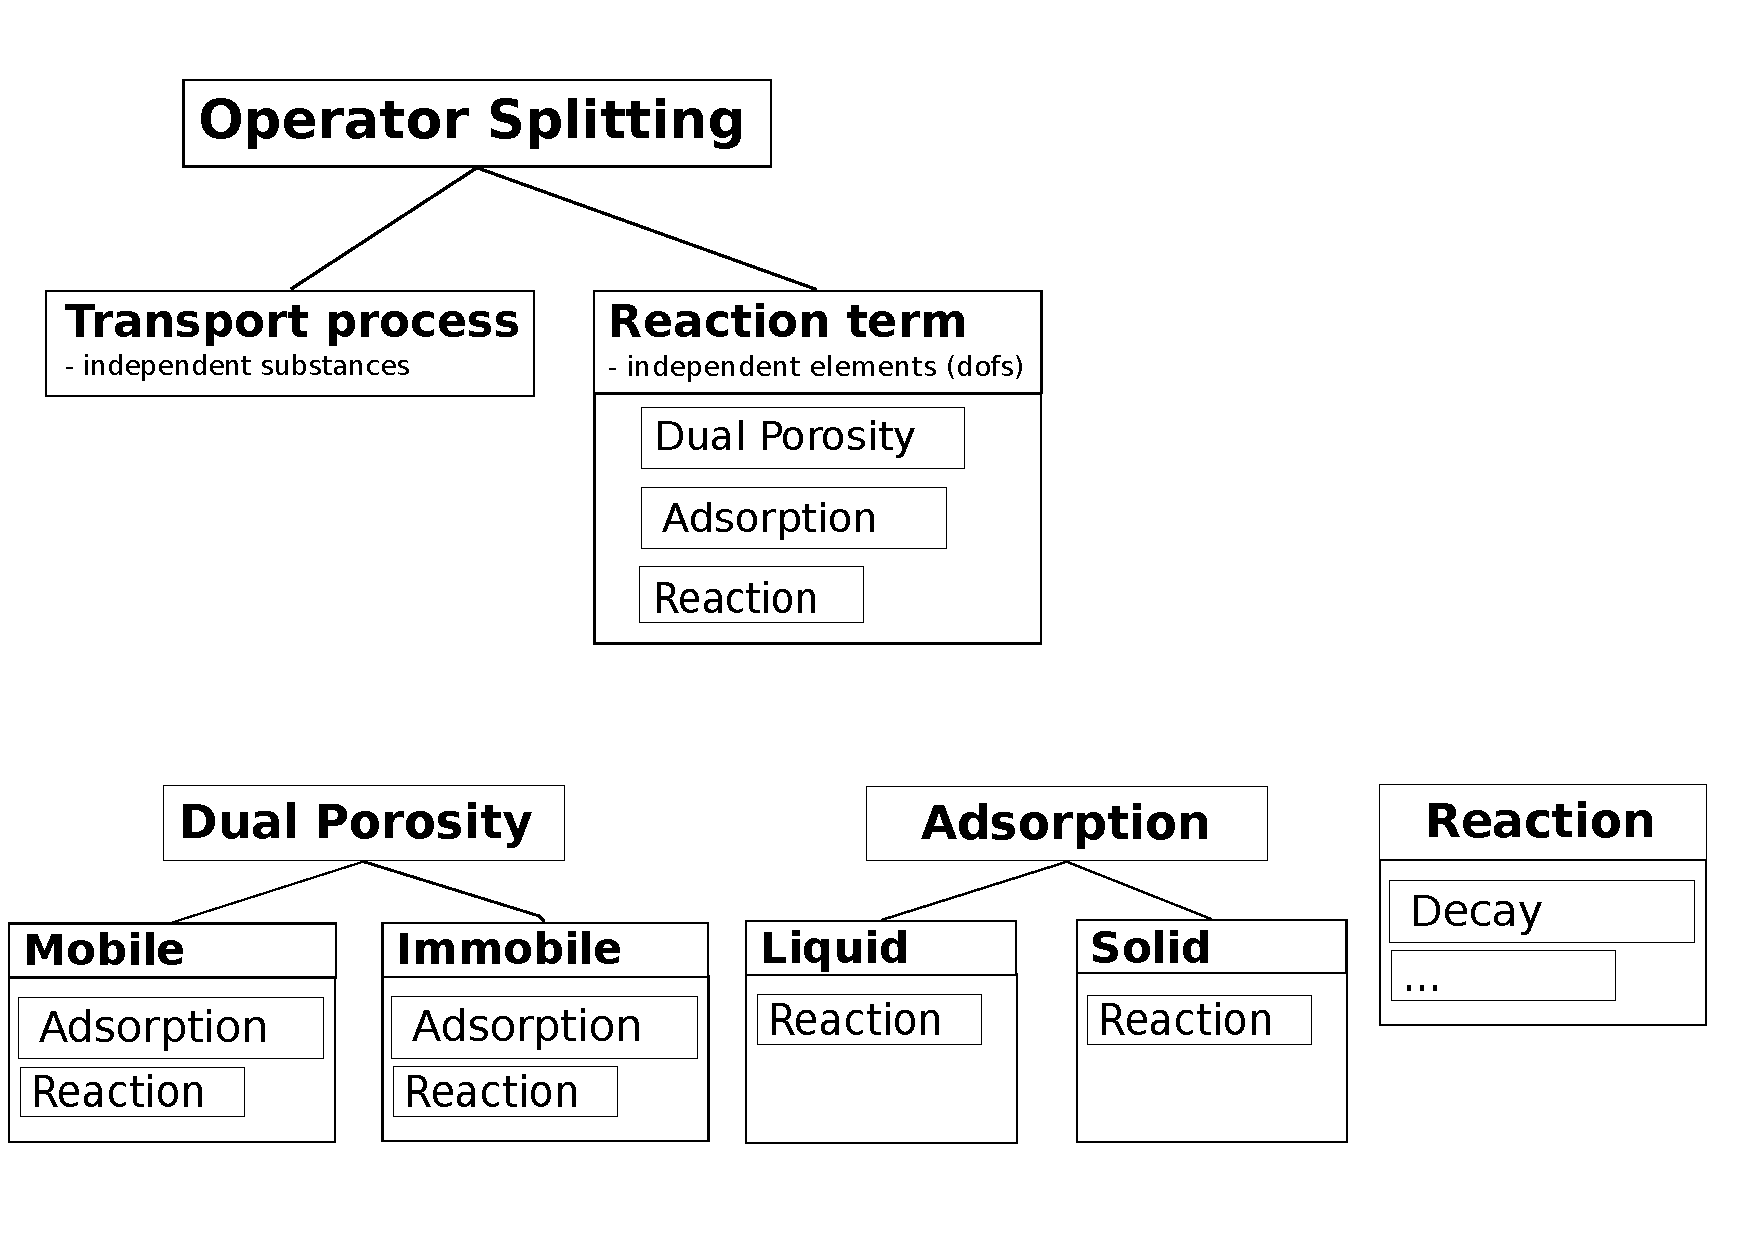
\includegraphics[width=\textwidth]{\fig/reaction_term.pdf}
  \caption{The scheme of the reaction term objects. The lines represents connections between different models. 
  The tables under model name include the possible models which can be connected to the model above.}
  \label{fig:reaction_term}
\end{figure}

The \emph{reaction} model acts only on the specified substances. It does not have its own output.

The \emph{adsorption} model describes the exchange of concentration of the substances between liquid and solid. It can be
followed by another \emph{reaction} that can run in both phases. The concentration in solid is an additional output 
of this model. See Subsection \ref{sec:sorp_math}.


The \emph{dual porosity} model, described in Subsection \ref{sec:dual_porosity}, introduces the so called immobile (or dead-end) pores in the matrix. The convection process operates only on the concentration of the substances in the mobile zone (open pores) 
and the exchange of concentrations from/to immobile zone is governed by molecular diffusion. This process can be followed by 
\emph{adsorption} model and/or chemical \emph{reaction}, both in mobile and immobile zone. The immobile concentration is an
additional output.


\subsection{Dual porosity}
\label{sec:dual_porosity}

Up to now we have described the transport equation for the single porosity model. The dual porosity model splits the mass into 
two zones -- the mobile zone and the immobile zone. Both occupy the same macroscopic volume, however on the microscopic scale, 
the immobile zone is formed by the dead-end pores, where the liquid is trapped and cannot pass through. The rest of the pore volume 
is occupied by the mobile zone. Since the liquid in the immobile pores is immobile, the exchange of the substance is only due 
to molecular diffusion. We consider simple nonequilibrium linear model:
\begin{align}
    \vartheta_m \partial_t c_m &= D_{dp} ( c_i - c_m), \label{eqn:dual_porosity_ode1}\\
    \vartheta_i \partial_t c_i &= D_{dp} ( c_m - c_i), \label{eqn:dual_porosity_ode2}
\end{align}
where $c_m$ is the concentration in the mobile zone, $c_i$ is the concentration in the immobile zone and
\hyperA{DualPorosity-Data::diffusion-rate-immobile}{$D_{dp}$} is a diffusion rate between the zones.
\hyperA{DualPorosity-Data::porosity-immobile}{$\vartheta_i$}~denotes porosity of the immobile zone  and 
$\hyperlink{TransportOperatorSplitting-Data::porosity::B}{\vartheta_m} = \vartheta$ the mobile porosity from transport equation \eqref{e:ADE}.

The analytical solution of the system of differential equations at time $t$ with initial conditions $c_m(0)$ and $c_i(0)$ is
\begin{align}
     c_m(t) &= (c_m(0) - c_a(0)) \exp\left(- D_{dp}\left(\frac{1}{\vartheta_m} + \frac{1}{\vartheta_i}\right) t \right) + c_a(0), \\
     c_i(t) &= (c_i(0) - c_a(0)) \exp\left(- D_{dp}\left(\frac{1}{\vartheta_m} + \frac{1}{\vartheta_i}\right) t \right) + c_a(0),
\end{align}
where $c_a$ is the weighted average
\[
  c_a = \frac{\vartheta_m c_m + \vartheta_i c_i}{\vartheta_m + \vartheta_i}.
\]

If the time step is large we use the analytical solution to compute new values of concentrations. 
Otherwise we replace the time derivatives in \eqref{eqn:dual_porosity_ode1} and \eqref{eqn:dual_porosity_ode2} 
by first order forward differences and we get the classical Euler scheme
\begin{align}
  c_m(t^+) = \frac{D_{dp} \Delta t}{\vartheta_m}(c_i(t) - c_m(t)) + c_m(t), \\
  c_i(t^+) = \frac{D_{dp} \Delta t}{\vartheta_i}(c_m(t) - c_i(t)) + c_i(t), \\
\end{align}
where $\Delta t = t^+ - t$ is the time step. 

\subsection{Equilibrial adsorption}
\label{sec:sorp_math}

The simulation of monolayer, equilibrial adsorption is based on the solution of two algebraic equations, namely the mass balance (in unit volume)
\begin{equation}
\label{eq:mass_balance_sorption}
\th \varrho_l c_l + (1-\th) \varrho_s M_s c_s = c_T = const.
\end{equation}
and an empirical adsorption law
\begin{equation}
\label{eq:relation_cs_cl}
c_s = f(c_l),
\end{equation}
given in terms of the so-called isotherm $f$.
Its form is determined by the parameter \hyperA{Sorption-Data::sorption-type}{\tt sorption\_type}:
\begin{itemize}
 \item ``$none$'': $f(c_l)=0$ (the adsorption model returns zero concentration in solid);
 \item ``$linear$'': $f(c_l) = k_l c_l$;
 \item ``$freundlich$'': $f(c_l) = k_F c_l^{\alpha}$;
 \item ``$langmuir$'': $f(c_l) = k_L \frac{\alpha c_l}{1 + \alpha c_l}$.
       Langmuir isotherm has been derived from thermodynamic laws. $k_L$ denotes the maximal amount 
       of sorbing specie which can be kept in an unit volume of a bulk matrix. Coefficient $\alpha$ is 
       a fraction of adsorption and desorption rate constant $\alpha = \frac{k_a}{k_d}$.
\end{itemize}

Notation:
\begin{itemize}
 \item Concentration in solid $c_s = \frac{n}{m_s}$ [mol\,$\mathrm{kg}^{-1}$], where $m_s$, $n$ is the 
       mass of solid and the molar amount of the substance in unit volume, respectively;
 \item Concentration in liquid $c_l = \frac{m}{m_l}$ \units{}{}{}, where $m_l$ is 
       the mass of liquid in unit volume. The relation between $c_l$ and the concentration $c$ from 
       transport equation \eqref{e:ADE} is $c = c_l \varrho_l$;
 \item \hyperA{Sorption::solvent-density}{$\varrho_l$}, \hyperA{Sorption-Data::rock-density}{$\varrho_s$} is the liquid (solvent) density and the solid (rock) density, respectively;
 \item \hyperA{Sorption::molar-mass}{$M_s$} denotes the molar mass of a substance;
 \item Multiplication parameters $k_i, i\in\{ l,F,L\}$ [mol\,$\mathrm{kg}^{-1}$] are given by 
       \hyperA{Sorption-Data::isotherm-mult}{\tt isotherm\_mult};
 \item Additional parameter $[\alpha] = 1$ is given by \hyperA{Sorption-Data::isotherm-other}{\tt isotherm\_other}.
\end{itemize}

Denoting
\[ \mu_l = \varrho_l \th, \quad \mu_s = M_s \varrho_s\cdot(1-\th), \]
and using \eqref{eq:relation_cs_cl}, the mass balance \eqref{eq:mass_balance_sorption} reduces to the equation
\begin{equation}
 c_T = \mu_l c_l + \mu_s f(c_l),
 \label{eq:nonlin_sorption}
\end{equation}
which can be either solved iteratively or using interpolation.
To solve \eqref{eq:nonlin_sorption} iteratively, it is very important to define the interval where 
to look for the solution (unknown $c_l$), see Figure \ref{fig:sorpce}. The lower bound is $0$ (concentration can not reach negative values). 
The upper bound is derived using a simple mapping. Let us suppose limmited 
\hyperA{Sorption::solubility}{$solubility$} of the selected transported substance and let us denote the 
limmit $\bar{c}_l$. We keep the maximal "total mass" 
$\bar{c}_T= \mu_l\cdot \bar{c}_l + \mu_s\cdot f(\bar{c}_l)$, but we dissolve all the mass to get 
maximal $c_l^{max} > \bar{c}_l$. That means $c_s = 0$ at this moment. We can slightly enlarge the interval by setting the upper bound equal to 
$c_l^{max} + const_{small}$.

\begin{figure}[ht!]
 \centering
 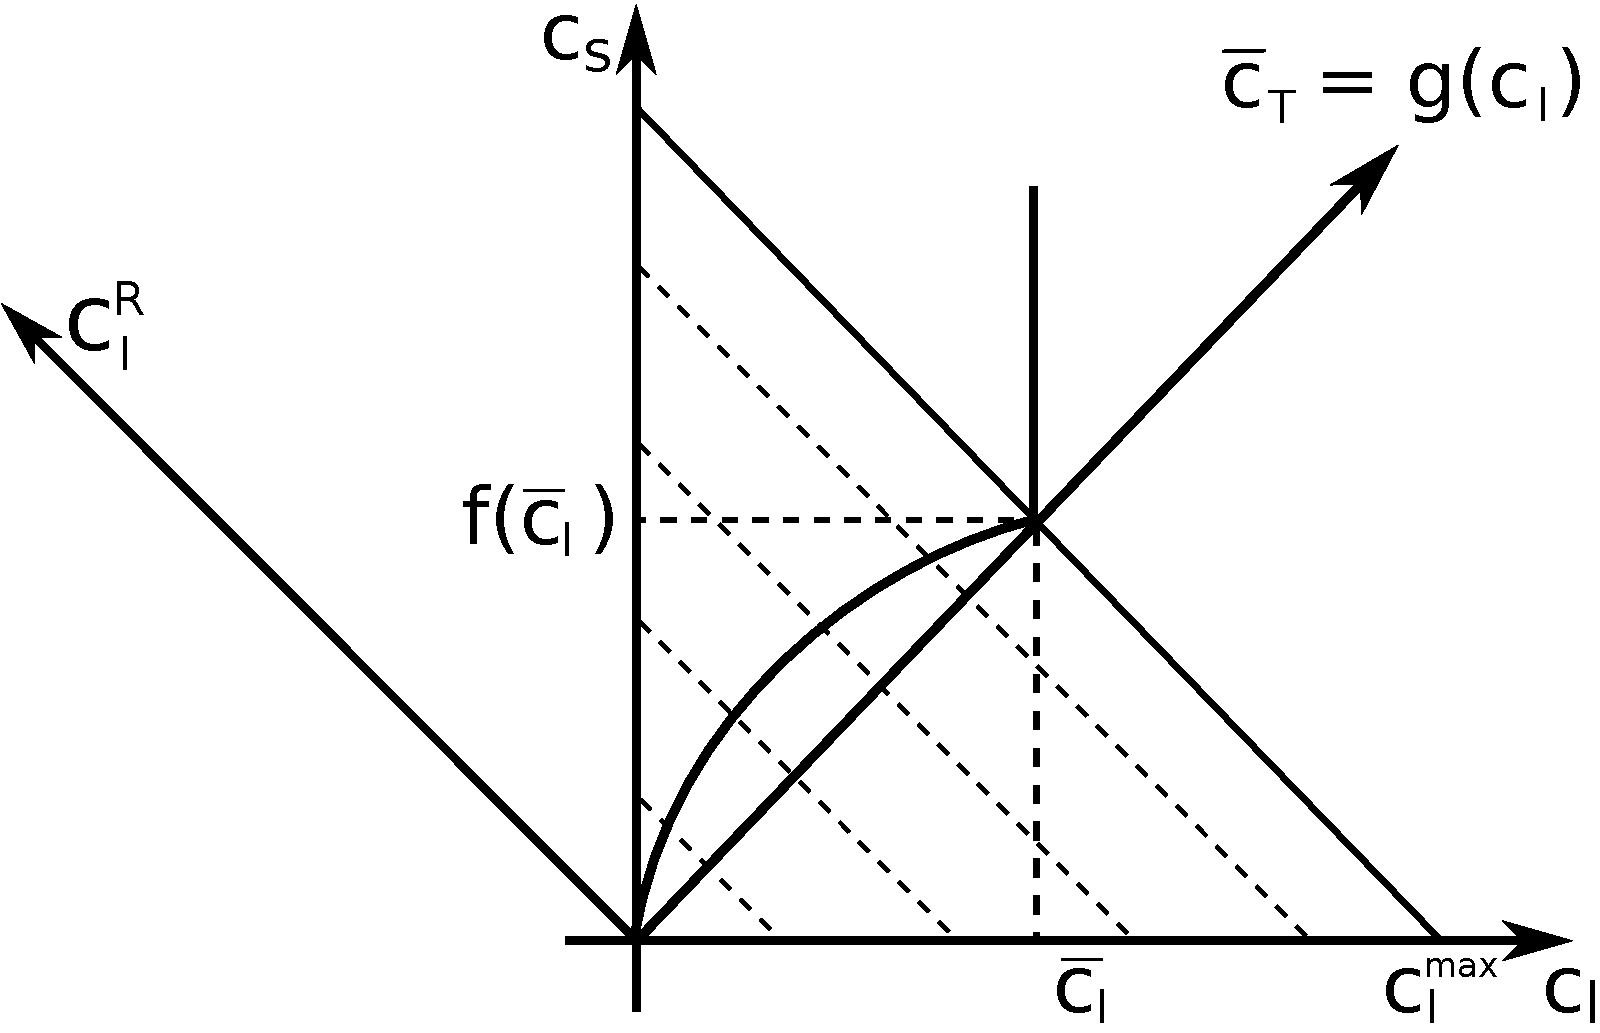
\includegraphics[width = 0.75\textwidth]{\fig/sorpce.pdf}
 \caption{Sorption in combination with limmited solubility.}
 \label{fig:sorpce}
\end{figure}


To approximate the equation \eqref{eq:nonlin_sorption} using interpolation we need to prepare the set of values 
which represent $[c_l, f(c_l)]$, with $c_l$ equidistantly distributed in transformed (rotated and rescaled) 
coordination system at first. The approach for construction of interpolation table follows.
\begin{enumerate}
 \item Maximal ``total mass'' $\bar{c}_T = \mu_l\cdot \bar{c}_l + \mu_s\cdot f(\bar{c}_l)$ is computed.
 \item Total mass step is derived $mass\_step = \bar{c}_T/n\_steps$. $n\_steps$ is given by
       \hyperA{Sorption::substeps}{$substeps$}.
 \item Appropriate $c_T^j = (mass\_step\cdot j)/\mu_l,~j\in \{0,\ldots, n\_steps\}$ are computed. 
 \item The equations $\mu_l \cdot c_T^j = \mu_l\cdot c_l^j + \mu_s\cdot f(c_l^j)~j\in \{0,\ldots, n\_steps\}$ are solved 
       for $c_l^j$ as unknowns. The solution is the set of ordered couples (points) 
       $[c_l^j,f(c_l^j)],~j\in\{0,\ldots,n\_steps\}$.
\end{enumerate}
After computation of $\{[c_l^j,f(c_l^j)]\}$ we transform these coordinates to the system where the total mass is 
an independent variable. This is done by multiplication of precomputed points using the transformation matrix ${\bf A}$:
\begin{equation}
 \begin{array}{l}
  \vec{c}\,^R = {\bf A}\cdot\vec{c}\\
  \left[\begin{array}{c} c_l^{R,j}\\ c_s^{R,j} \end{array}\right] = 
  \left[\begin{array}{cc}
    \vartheta\cdot \rho_w & M_s(1 - \vartheta)\rho_R\\
    -M_s(1 - \vartheta)\rho_R & \vartheta\cdot \rho_w
  \end{array}\right]\cdot
  \left[\begin{array}{c} c_l^j\\ c_s^j \end{array}\right]\\
  j\in\{0,\ldots,n\_steps\}
 \end{array}
 \label{eq:transf_mat}
\end{equation}

The values $c_l^{R,j}$ are equidistantly distributed and there is no reason to save them, but the values 
$c_s^{R,j}$ are stored in onedimensional interpolation table.

Once we have the interpolation table, we can use it for projection of ${[c_l,c_s]}$ transport results on the 
isotherm under consideration. The approach looks as folows.
\begin{enumerate}
 \item Achieved concentrations are transformed to the coordinate system through multiplication with the 
       matrix ${\bf A}$, see \eqref{eq:transf_mat}.
 \item Transformed values are interpolated.
 \item The result of interpolation is transformed back. The backward transformation consist of multiplication 
       with ${\bf A}^T$ which is followed by rescaling the result. Rescaling the result is necessary because  
       ${\bf A}$ is not orthonormal as it is shown bellow.
 \[
 \begin{array}{l}
 {\bf A}^T\cdot{\bf A} =
  \left((\vartheta - 1)^2\cdot M_s^2\cdot \rho_R^2 + \vartheta^2\cdot \rho_w^2\right)\cdot\left[\begin{array}{cc}
    1 & 0\\
    0 & 1
  \end{array}\right]
  \end{array}
 \]
\end{enumerate}


\subsection{Limited solubility}\label{subsec:lim_solub}
When $\mu_l\cdot c_l + \mu_s\cdot f(c_l) > \mu_l\cdot \bar{c}_l + \mu_s\cdot f(\bar{c}_l)$ neither iterative 
solver nor interpolation table is used. The aqueous concentration is set to be $\bar{c}_l$ and sorbed 
concentration is computed $c_s = (\mu_l\cdot c_l + \mu_s\cdot f(c_l) - \mu_l\cdot \bar{c}_l)/\mu_s$.

\subsection{Sorption in dual porosity model} 
\label{subsec:sorp_dual_por}
There are two parameters $\mu_l$ and $\mu_s$, scale of aqueous concentration and scale of sorbed concentration, respectively.  
There is a difference in computation of these in the dual porosity model because both work on different concentrations
and different zones.

Let $c_{ml}$ and $c_{ms}$ be concentration in liquid and in solid in the mobile zone, 
$c_{il}$ and $c_{is}$ be concentration in liquid and in solid in the immobile zone,
$\vartheta_m$ and $\vartheta_i$ be the mobile and the immobile porosity,
and $\varphi$ be the sorbing surface.

The sorbing surface in the mobile zone is given by
\begin{equation}
  \varphi = \frac{\vartheta_m}{\vartheta_m + \vartheta_i}, 
\end{equation}

while in the immobile zone it becomes
\[ 1 - \varphi = 1-\frac{\vartheta_m}{\vartheta_m + \vartheta_i} = \frac{\vartheta_i}{\vartheta_m + \vartheta_i}. \]

Remind the mass balance equation \eqref{eq:nonlin_sorption}.
In the dual porosity model, the scaling parameters $\mu_l$, $\mu_s$ are slightly different.
In particular, the mass balance in the mobile zone reads:
\begin{eqnarray}
 \begin{array}{l}
  c_T = \mu_l\cdot c_{ml} + \mu_s\cdot c_{ms},\\
  \mu_l = \varrho_l \cdot \vartheta_m, \\
  \mu_s = M_s \cdot\varrho_s\cdot(1-\vartheta_m - \vartheta_i)\varphi,
 \end{array}
 \label{eq:scale_params_m}
\end{eqnarray}
while in the immobile zone it has the form:
\begin{eqnarray}
 \begin{array}{l}
  c_T = \mu_l\cdot c_{il} + \mu_s\cdot c_{is},\\
  \mu_l = \varrho_l \cdot \vartheta_i, \\
  \mu_s = M_s \cdot\varrho_s\cdot(1-\vartheta_m - \vartheta_i)(1 - \varphi).
 \end{array}
 \label{eq:scale_params_i}
\end{eqnarray}
